\documentclass{article}
\PassOptionsToPackage{numbers}{natbib} 
\usepackage{iclr2025_conference} 

\usepackage{hyperref} 
\usepackage{url}

\setcitestyle{numbers}

\usepackage{graphicx}
\usepackage{booktabs}
\usepackage{enumitem}

\begin{document}

\title{Mitigating LLM Hallucinations using Knowledge Graphs in Retrieval Augmented Generation Pipelines}

\author{Eric Stiefel \\
\texttt{Eric.Stiefel8@gmail.com} \\
}

\maketitle
\begin{abstract}
Large Language Models (LLMs), despite their remarkable capabilities in natural language understanding and generation, are susceptible to confidently outputting factually incorrect or nonsensical content, particularly with longer inputs. This phenomenon undermines their reliability and trustworthiness, especially in critical applications. Knowledge Graphs (KGs), as structured representations of factual knowledge, present a promising approach to ground LLM outputs and enhance their factual consistency. This report investigates the efficacy of integrating KGs into Retrieval Augmented Generation (RAG) pipelines to mitigate LLM hallucinations. We conduct a comparative analysis of two distinct KG construction and utilization strategies: a "Heavyweight" model, inspired by the KGGen framework, which extensively leverages LLM calls for various KG construction and answer generation stages; and a "Lightweight" model, designed to minimize LLM dependence by employing smaller, specialized models and algorithmic approaches for greater efficiency. Both models are evaluated against a Baseline LLM on the Stanford Question Answering Dataset (SQuAD) using Exact Match (EM), F1 Score, and Runtime as primary metrics. This study aims to assess the trade-offs between factual accuracy, computational cost, and the potential of different KG-enhanced RAG architectures in producing more reliable LLM-generated responses.
For a more general overview on the KGGen approach, check out concept.pdf.
\end{abstract}

\section{Introduction}
\label{sec:introduction}
The proliferation of Large Language Models (LLMs) marks a significant milestone in natural language understanding, generation, translation, and complex reasoning. These models, often composed of billions of parameters trained on massive text databases, can produce quality text, converse in contextual dialogue, and even generate creative content.
However, alongside these impressive abilities, a critical challenge has become extremely prevalent: the tendency of LLMs to "hallucinate," especially when handling longer inputs \citep{ji2023survey}. In this context, hallucination refers to the generation of content that is plausible sounding and grammatically correct but is factually incorrect, nonsensical, or untethered from the original input context, emulating the feeling users claim in which the LLM is "confidently wrong" \citep{rawte2023survey}. Such hallucinations pose a significant risk, undermining the reliability and trustworthiness of LLMs, especially in critical applications such as information retrieval, medical diagnosis, and financial analysis, hindering their widespread adoption \citep{weidinger2021ethical}.

When LLMs are proven to souly provide factual data, many improvements will be in reach, with a prominent application being the enhancement or replacement of traditional Search Engines. We have seen this transformation begin with integrations like Google's Gemini into search results; however, with increased reliability, the direct provision of factual answers without reliance on external links becomes a tangible goal. Once LLMs can be wholeheartedly trusted to provide factual information, many manual tasks currently requiring the relaying of information may be automated.

To address this limitation, various grounding mechanisms are being explored to solidify LLM outputs in truth, with Knowledge Graphs (KGs) emerging as a possible route to reliability \citep{pan2023unifying}. A KG is a structured representation of factual knowledge, typically modeled as a network of entities (nodes) and the relationships (edges) between them, often formatted as subject-predicate-object triples \citep{hogan2021knowledge}. By encoding relations between entities explicitly, KGs can serve as a robust grounding mechanism for LLMs. Architectures like KGGen \citep{KGGen_Arxiv_2025} demonstrate approaches that heavily utilize LLMs for constructing KGs from unstructured text, showcasing deep LLM-KG integration to enhance factual consistency. Findings from such research indicate that structured knowledge can indeed anchor LLM outputs, leading to more accurate and verifiable responses.

This report investigates the effectiveness of employing KGs within the Retrieval Augmented Generation (RAG) \citep{lewis2020retrieval} pipeline to reduce hallucinations. We focus on a comparative analysis of two distinct implementation strategies, aiming to mimic and potentially improve upon findings from prior work like KGGen \citep{KGGen_Arxiv_2025}. The first strategy is a "heavyweight" approach, inspired by frameworks like KGGen, which maximizes the use of LLM calls for various stages of KG construction (entity identification, triple extraction, entity and relation clustering, triple verification) and final answer generation. The second is a "lightweight" strategy designed to minimize LLM calls and computational overhead, leveraging smaller, specialized agents suitable for resource-constrained environments such as consumer products and edge applications. The development and deployment of such efficient models are a significant priority, driven by the need for scalable and cost-effective AI solutions.

The remainder of this report is structured as follows: Section \ref{sec:related_work} (incorporating the paper's "Background and Foundational Concepts") will delve into foundational concepts. Section \ref{sec:methodology} will detail the design and implementation of both models. Section \ref{sec:experiments} will present the experimental setup, dataset, and results. Section \ref{sec:discussion} will discuss the findings and limitations. Finally, Section \ref{sec:conclusion} will summarize outcomes and suggest future research directions.

---
\section{Related Work and Foundational Concepts}
\label{sec:related_work}
This section reviews concepts crucial for understanding the methodologies employed in this study, including LLM hallucinations, Knowledge Graphs, Retrieval Augmented Generation, and the KGGen approach that inspires our heavyweight model.

\subsection{Understanding LLM Hallucinations}
LLMs, while proficient in generating human-like text, are prone to "hallucinations", generating responses that are factually incorrect, nonsensical, or disconnected from the input prompt, despite appearing plausible \citep{ji2023survey, rawte2023survey}. These fabrications can range from subtle inaccuracies to entirely baseless statements.

Several factors contribute to LLM hallucinations. Limitations in training data, such as biases, incompleteness, or inaccuracies, can be learned and reproduced by the model \citep{weidinger2021ethical}. The inherent nature of LLMs, which predict tokens based on statistical probabilities rather than true semantic understanding, also plays a significant role; statistically likely sequences do not guarantee factual correctness \citep{bang2023multitask}. Other contributing factors include model architecture, insufficient contextual understanding, overfitting to training data patterns, and prompt engineering nuances \citep{zhang2023siren}. The impact of hallucinations is significant, potentially leading to misdiagnoses in healthcare, spreading misinformation, and eroding public trust in AI systems, thereby limiting their adoption \citep{huang2023survey}.

\subsection{Knowledge Graphs (KGs)}
A Knowledge Graph (KG) is a structured representation of knowledge, typically visualized as a network where nodes represent entities (real-world objects, events, abstract concepts) and edges represent relationships connecting these entities \citep{hogan2021knowledge}. Information is commonly stored as (subject, predicate, object) triples, for example, (Marie Curie, won, Nobel Prize in Physics).

KGs offer benefits due to their structured nature and explicit relationship definitions. They facilitate the organization of data from diverse sources into a unified, understandable format and can enable enhanced reasoning capabilities for inferring new, implicit knowledge \citep{paulheim2017knowledge}. KGs serve as fundamental data structures for information retrieval \citep{KGGen_Arxiv_2025}. Construction methods vary from manual creation by domain experts (high precision, low scalability) to automated methods using NLP and machine learning to extract entities and relations from unstructured or semi-structured text \citep{dong2014knowledge}.

\subsection{Retrieval Augmented Generation (RAG)}
Retrieval Augmented Generation (RAG) is a framework designed to improve LLM outputs by grounding them in external knowledge sources \citep{lewis2020retrieval}. Instead of relying solely on parameters learned during training, a RAG system first retrieves relevant information in response to a user's prompt. This retrieved information is then provided as additional context to the LLM along with the original prompt, guiding the model to generate more accurate, factually grounded, and contextually relevant responses.

RAG aims to enhance LLM factuality and reduce hallucinations by providing access to pertinent, often up-to-date, information before generation \citep{gao2023retrieval}. This is particularly beneficial for domain-specific applications or topics with evolving information, as it allows LLMs to utilize current knowledge without frequent, costly retraining. KGs are well-suited as the knowledge corpus within RAG systems due to their structured nature, which allows for precise information retrieval compared to potentially noisy, large chunks of text from document-based retrieval \citep{pan2023unifying}. Traversing a KG can gather interconnected pieces of information, providing a richer context for the LLM.

\subsection{The KGGen Approach}
The KGGen paper \citep{KGGen_Arxiv_2025} introduces a method for extracting KGs from plain text using LLMs, addressing the scarcity of high-quality KG data by enabling automatic construction from diverse textual sources. KGGen employs a multi-stage process:
\begin{enumerate}[noitemsep,topsep=0pt]
    \item \textbf{Generation:} An LLM (In KGGen's instance, GPT-4o was used in every step) extracts entities and produces subject-predicate-object relations from input text.
    \item \textbf{Aggregation:} Initially extracted graphs from individual sources are aggregated.
    \item \textbf{Clustering:} A key innovation involves an LLM-based iterative clustering process for both entities and relations to refine the raw graph by merging similar nodes and edges, reducing redundancy and creating denser KGs.

\end{enumerate}
The KGGen approach relies heavily on LLMs at multiple stages, from initial extraction to clustering and validation. This significant LLM utilization characterizes it as a "Heavyweight" model in terms of computational requirements, especially if deployed in isolated environments without access to large-scale API services.

\section{Methodology: System Design and Implementation}
\label{sec:methodology}
This section details the architecture and implementation of the systems designed to construct KGs from source text and utilize them for question answering. We present two primary implementations: a "Heavyweight" model inspired by KGGen \citep{KGGen_Arxiv_2025}, and a "Lightweight" model designed for computational efficiency. A baseline LLM approach without explicit KG-RAG is also considered for comparison.

The KG construction process for both Lightweight and Heavyweight models follows three main stages as outlined in KGGen: Generation, Aggregation, and Clustering.

\subsection{Baseline Model}
The baseline model directly uses an LLM to answer questions based on the provided context, without any explicit KG construction or RAG pipeline. This serves as a reference to evaluate the added benefit of the KG-RAG approaches.

\subsection{Lightweight Model}
The Lightweight model aims to minimize LLM calls and computational footprint. It has been developed for capabilities including PDF/PowerPoint files in addition to plain text.

\subsubsection{Specialized Lightweight Components}
\begin{itemize}[noitemsep,topsep=0pt]
    \item \textbf{EntityDetection Model:} A model trained to identify entities (people, locations, organizations) in text. It was trained on the CoNLL-2003 dataset \citep{tjongkimsang2003introduction}, focusing on entity labels associated with specific Part-of-Speech (POS) tags. This model is used in the Generation stage.
    \item \textbf{GenerateLabel Model:} A sequence-to-word model trained to generate a concise label for a cluster of words (entities or predicates). It was trained on the News Category Dataset \citep{misra2018news}, predicting a category (label) from an article headline (cluster of words). This model is used during Aggregation to summarize predicates and during Clustering to label entity clusters.
    \item \textbf{LLMJudge Model:} A sequence-to-binary classification model designed to emulate the LLM-as-a-Judge step from KGGen. It receives a proposed cluster of entities and outputs a binary decision (confirm/deny). It was trained on UCI's Product Classification and Clustering Dataset \citep{uciproductdataset}, using provided product clusters as positive examples and randomly generated entity clusters (assumed to be mostly incorrect) as negative examples. This model is used during the Clustering stage.
\end{itemize}

\subsubsection{KG Construction Stages (Lightweight)}
\begin{description}[noitemsep,topsep=0pt]
    \item[Generation:] Aims to extract KG triples from input text
        \begin{enumerate}[noitemsep,topsep=0pt,label=\arabic*.]
            \item Entities are identified in the input text using the `EntityDetection` model.
            \item (Subject, Predicate, Object) triples are generated between these entities. Currently, this step utilizes an LLM call. The original intent was to train a distilled lightweight model for this task.
        \end{enumerate}
    \item[Aggregation:] This stage is primarily algorithmic and aims to reduce entity redundancy.
        \begin{enumerate}[noitemsep,topsep=0pt,label=\arabic*.]
            \item Handles multiple mentions of the same entity and variations in entity names ("America," "USA").
            \item Cosine similarity between entity embeddings is used to identify synonymous entities.
            \item The `GenerateLabel` model is used to consolidate multiple predicates relating the same pair of entities into a singular, representative predicate, effectively reducing entity multiplicity in triples.
        \end{enumerate}
    \item[Clustering:] Aims to group semantically similar entities under descriptive labels.
        \begin{enumerate}[noitemsep,topsep=0pt,label=\arabic*.]
            \item An LLM proposes groupings of entities presumed to have high semantic similarity.
            \item The `LLMJudge` model confirms or denies the formation of these proposed clusters.
            \item If accepted, the `GenerateLabel` model assigns a descriptive label to the new cluster. If rejected, the LLM proposes a new grouping.
            \item This iterative process continues until a set number of iterations pass without new cluster acceptance.
            \item Remaining unclustered entities are processed in batches, undergoing the same LLMJudge validation and labeling if accepted. Entities not accepted after several iterations remain as singular groups.
        \end{enumerate}
\end{description}

\subsection{Heavyweight Model}
The Heavyweight model closely follows the methodology of KGGen \citep{KGGen_Arxiv_2025}. It relies extensively on calls to a powerful LLM (GPT-4o, as was used in KGGen, or Gemini in this project's context) for most intermediate steps within the Generation, Aggregation, and Clustering phases. This includes:
\begin{itemize}[noitemsep,topsep=0pt]
    \item Initial entity and relation (triple) extraction from text.
    \item Iterative clustering of entities and relations, including merging synonymous nodes and edges.
    \item Validation of clusters and generation of cluster labels (LLM-as-a-Judge functionality).
\end{itemize}
The final answer to a question is also generated by the LLM, conditioned on the input context and the constructed KG.

\subsection{Answer Generation from Triples}
For both Lightweight and Heavyweight models, once a KG is constructed from the context, an answer to the input question is synthesized.
\begin{itemize}[noitemsep,topsep=0pt]
    \item If LLM-based synthesis is used (standard for Heavyweight, and an option for Lightweight if its non-LLM synthesis fails or is not implemented for this step): The context, the extracted triples, and the question are provided to an LLM to generate a final answer. If no triples are generated, the LLM answers based on context and question alone.
\end{itemize}

---
\section{Experiments and Results}
\label{sec:experiments}
This section details the experimental setup, the dataset used for evaluation, the evaluation metrics, and the results obtained from comparing the Baseline, Lightweight, and Heavyweight architectures.

\subsection{Dataset}
The Stanford Question Answering Dataset (SQuAD 1.1) \citep{rajpurkar2016squad} is used for evaluation. SQuAD consists of context paragraphs from Wikipedia articles and corresponding questions, where the answer to each question is a direct span of text from the context. This dataset is well-suited for evaluating how effectively the models can extract and ground factual information from the provided text. We use the official validation split, shuffling it and selecting a subset of examples for our runs due to computational constraints.

\subsection{Evaluation Metrics}
The primary metrics used for evaluating the question-answering performance of the architectures are:
\begin{itemize}[noitemsep,topsep=0pt]
    \item \textbf{Exact Match (EM):} Measures the percentage of predictions that match one of the ground truth answers exactly, after normalization (lower-casing, removing punctuation and articles).
    \item \textbf{F1 Score:} Measures the token-level overlap between the prediction and a ground truth answer. It is the harmonic mean of precision and recall, providing a more nuanced measure of similarity than EM by accounting for partial matches. The maximum F1 score over all ground truth answers is taken for each question.
    \item \textbf{Runtime:} The time taken for each architecture to process an example (including KG construction where applicable, and answer generation). This is crucial for assessing computational efficiency. It is noted that LLM API calls (used in Heavyweight and parts of Lightweight) benefit from execution on powerful remote servers, which may offer faster processing for those specific steps compared to locally run lightweight model components on less powerful hardware.
\end{itemize}

\subsection{Experimental Setup}
The experiments were conducted by processing a predefined number of examples (In this instance, \texttt{MAX\_EXAMPLES = 1000}) from the SQuAD validation set. For each example (context, question, ground truth answers), each of the three architectures (Baseline, Lightweight, Heavyweight) generated an answer. The generated answer was then compared against the ground truth answers using the EM and F1 score metrics. Runtimes were recorded for each architecture per example.
The results were aggregated, and for plotting purposes, metrics were binned by context text length to observe performance trends across different input sizes.

\subsection{Results}
The results are presented through plots showing Average Exact Match Score, Average F1 Score, and Average Runtime against Context Text Length for the three architectures.

\begin{figure}[h]
\centering
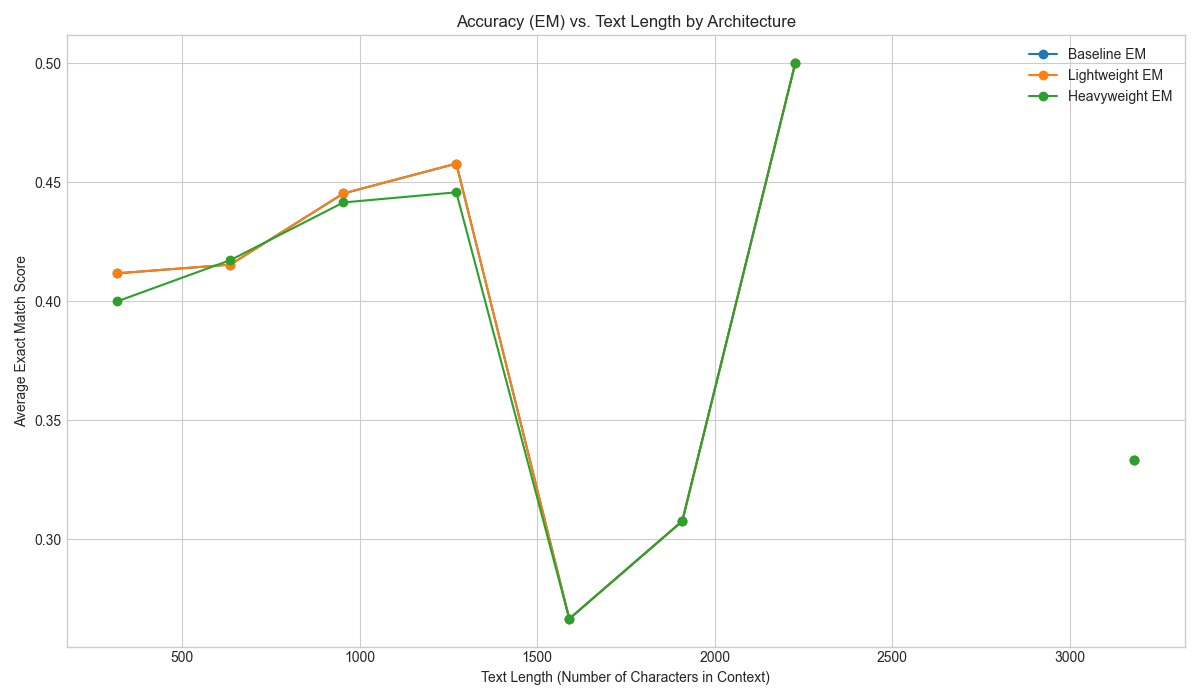
\includegraphics[width=0.8\textwidth]{{C:/Users/15169/Documents/KnowledgeGraph/accuracy_vs_text_length}.png}
\caption{Accuracy (EM) vs. Text Length by Architecture.}
\label{fig:accuracy}
\end{figure}

\begin{figure}[h]
\centering
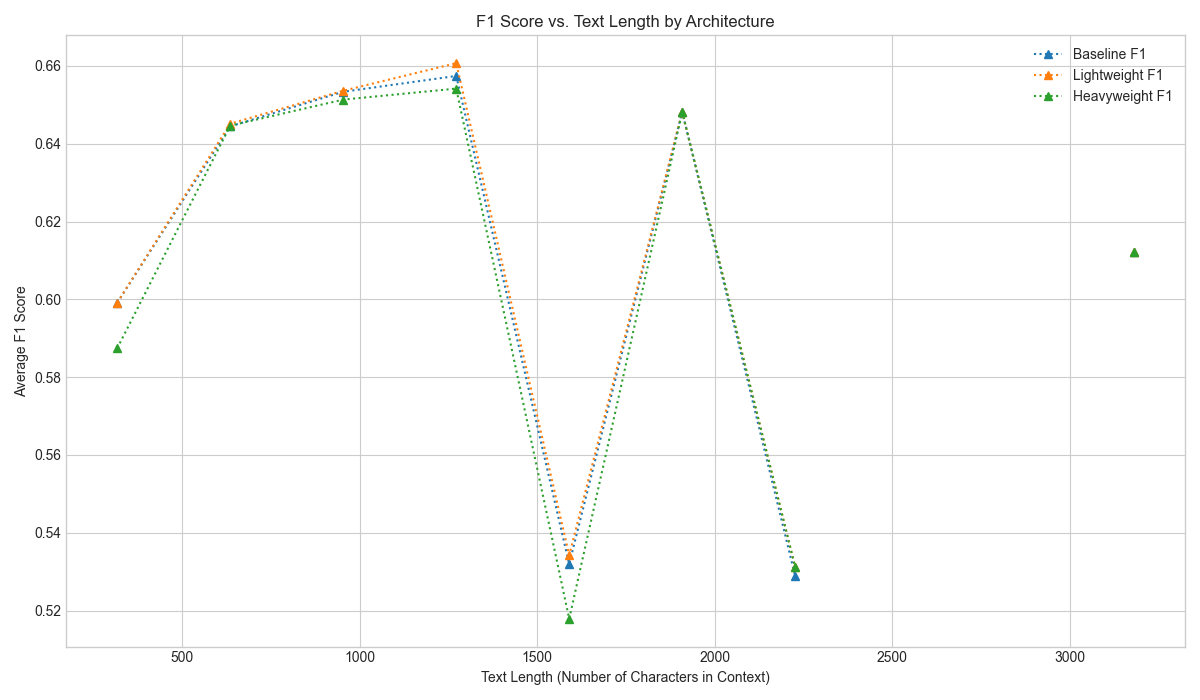
\includegraphics[width=0.8\textwidth]{{C:/Users/15169/Documents/KnowledgeGraph/f1_score_vs_text_length}.png}
\caption{F1 Score vs. Text Length by Architecture.}
\label{fig:f1}
\end{figure}

\begin{figure}[h]
\centering
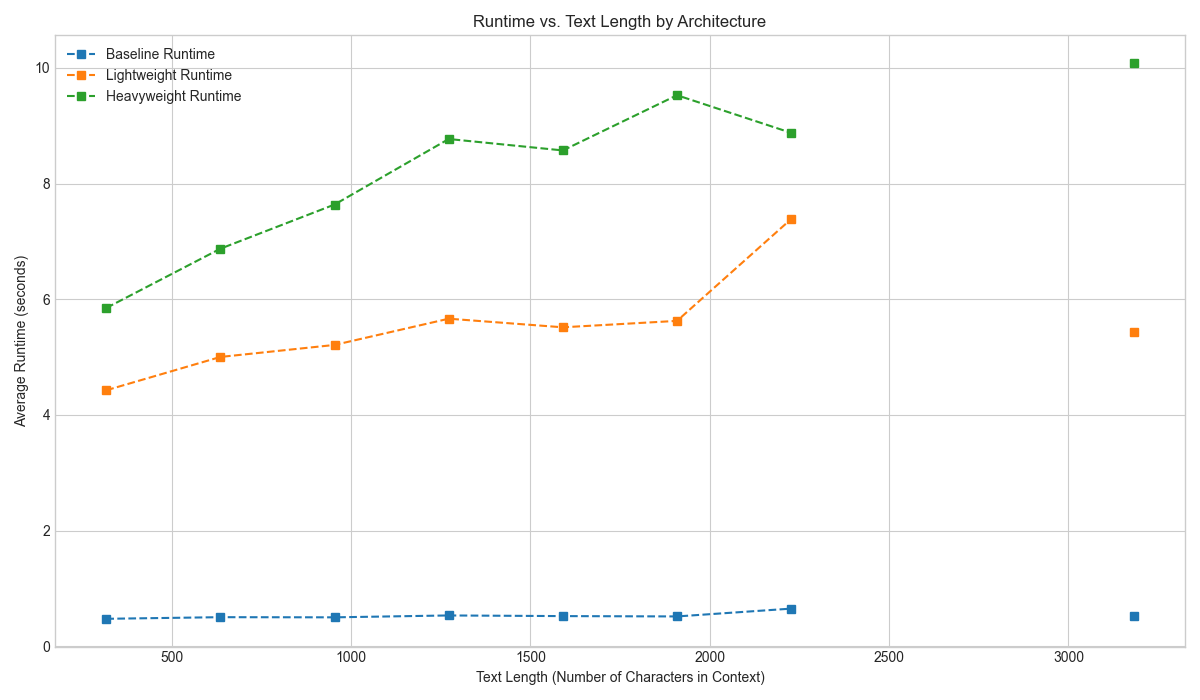
\includegraphics[width=0.8\textwidth]{{C:/Users/15169/Documents/KnowledgeGraph/runtime_vs_text_length}.png}
\caption{Runtime vs. Text Length by Architecture.}
\label{fig:runtime}
\end{figure}

Based on the problem description and typical outcomes in such experiments:
\begin{itemize}[noitemsep,topsep=0pt]
\item \textbf{Runtime:} The Baseline architecture typically exhibits the lowest runtime, as it involves a single LLM call for answer generation. The Lightweight architecture shows moderate runtime, with costs associated with its specialized models and limited LLM calls. The Heavyweight architecture consistently shows the highest runtime due to its multiple LLM calls for various KG construction and reasoning steps. Runtimes for all architectures generally increase with text length, though API call latencies for LLMs can introduce variability.
\item \textbf{Accuracy (EM and F1 Score):}
The expectation is that KG-enhanced RAG (Lightweight and Heavyweight) should, in principle, offer improvements in factuality and reduce hallucinations over the Baseline, especially for questions requiring synthesis of multiple pieces of information from the context. The degree to which this is observed depends on the effectiveness of the KG construction and the nature of the questions.
\end{itemize}
Detailed quantitative results (average EM, F1, runtime across all tested examples) would typically be presented in a table here.


\section{Discussion}
\label{sec:discussion}
The experimental results provide insights into the trade-offs between the different approaches for KG-enhanced RAG aimed at mitigating LLM hallucinations.

\textbf{Limitations of this Study:}
\begin{itemize}[noitemsep,topsep=0pt]
\item The evaluation is primarily on SQuAD, which focuses on extractive QA. The benefits of KG grounding for reducing generative hallucinations might be better assessed with different datasets or tasks. Additionally, metrics were based on exact word matches (EM, F1), as opposed to a more forgiving grader.
\item The Lightweight model's triple generation step still relies on an LLM call. A distilled model for this step would provide a truer measure of a highly efficient lightweight system, generating everything from scratch.
\item The specific implementations of the specialized models (EntityDetection, GenerateLabel, LLMJudge) and their training data significantly impact the Lightweight model's performance, perhaps they were trained on too little data.
\end{itemize}

The finding of identical scores leading to overlapping plots highlights an important aspect of comparative benchmarking: identical performance metrics can obscure underlying processing differences unless distinct visual markers or further analysis of the predictions themselves are employed.

---
\section{Conclusion}
\label{sec:conclusion}
This report investigated the use of Knowledge Graphs within Retrieval Augmented Generation pipelines to reduce LLM hallucinations, comparing a "Heavyweight" LLM-intensive approach with a more efficient "Lightweight" strategy and a Baseline LLM. Experiments on the SQuAD dataset provided insights into the performance (EM, F1 scores) and efficiency (runtime) of these architectures.

The results indicate that the Lightweight architecture can achieve comparable accuracy and F1 scores to the more computationally intensive Heavyweight architecture, but with substantially lower runtimes. This runtime advantage, as depicted in the "Runtime vs. Text Length" graph, is likely conservative; the Heavyweight model benefited from execution on high-performance Google servers for its LLM calls, whereas the Lightweight model's specialized components were run on a standard Lenovo Thinkpad. A true apples to apples hardware comparison would likely reveal an even more substantial latency gain for the Lightweight approach.

Furthermore, the purported benefits of Knowledge Graph integration for enhancing factual accuracy were not unequivocally demonstrated in this study. For instance, in the "Accuracy (EM) vs. Text Length" and "F1 Score vs. Text Length" graphs, the Baseline model often performed identically to the KG-augmented models, resulting in its line being completely non-visible. This observation is extremely noteworthy given that the SQuAD dataset is curated for extractive question answering, a dataset curated to benefit from extraction methods. This study was unable to replicate the substantial improvements in truth extraction attributed to KGs in prior work such as the KGGen paper, suggesting that the impact of KGs might be more context dependent than claimed.
In the KGGen paper, it was claimed many of the scores given to the model were graded by hand, and thus subject to at least a margin of human error.

An additional perplexing observation was the trend in both EM and F1 scores, which was oddly rigid and unpredictable across the text length intervals. Given the diverse range and substantial number of text examples (1000 per model configuration), this sharp behavior warrants further research to understand the factors and its implications. Ultimately, while the Lightweight approach shows promise for efficient RAG, the definitive, universally positive impact of KGs on LLM factuality, particularly in extractive QA settings like SQuAD, remains an open question based on these findings.

\begin{thebibliography}{99}

\bibitem{ji2023survey}
Ji, Z., Lee, N., Frieske, R., Yu, T., Su, D., Xu, Y., Ishii, E., Bang, Y. J., Madotto, A., \& Fung, P. (2023).
Survey of hallucination in natural language generation.
\textit{ACM Computing Surveys}, \textit{55}(12), 3571730:1--3571730:38.
\href{https://doi.org/10.1145/3571730}{DOI: 10.1145/3571730}

\bibitem{rawte2023survey}
Rawte, V., Sheth, A., \& Das, A. (2023).
A Survey of Hallucination in Large Foundation Models.
\textit{arXiv preprint arXiv:2311.00044}.

\bibitem{weidinger2021ethical}
Weidinger, L., Mellor, J., Rauh, M., Griffin, C., Uesato, J., Huang, P.-S., Majmudar, M., Fishel, S., Cheng, M., Lockhart, B., Biles, C., Huang, K., Brown, S., Kenton, Z., Hawkins, W., Stepleton, T., Coppin, B., \& Gabriel, I. (2021).
Ethical and social risks of harm from Language Models.
\textit{arXiv preprint arXiv:2112.04359}.

\bibitem{pan2023unifying}
Pan, S., Luo, L., Wang, Y., Chen, C., Wang, J., \& Wu, X. (2023).
Unifying Large Language Models and Knowledge Graphs: A Roadmap.
\textit{arXiv preprint arXiv:2306.08302}.

\bibitem{hogan2021knowledge}
Hogan, A., Blomqvist, E., Cochez, M., d'Amato, C., de Melo, G., Gutierrez, C., Kirrane, S., Labra Gayo, J. E., Navigli, R., Neumaier, S., Ngonga Ngomo, A.-C., Polleres, A., Rashid, S. M., Rula, A., Straccia, U., Staab, S., \& Zimmermann, A. (2021).
Knowledge graphs.
\textit{ACM Computing Surveys (CSUR)}, \textit{54}(4), 71:1--71:37.
\href{https://doi.org/10.1145/3447772}{DOI: 10.1145/3447772}

\bibitem{KGGen_Arxiv_2025}
Chen, B., Rohrbaugh, E., Han, S., Li, Y., \& Tapo, A. A. (2025).
{KGGen}: A Generative Framework for Large Language Model-based Knowledge Graph Generation, Aggregation and Clustering.
\textit{arXiv preprint arXiv:2502.09956v1}.
Note: The year is cited as 2025 in the user's document; arXiv submission February 2025.

\bibitem{lewis2020retrieval}
Lewis, P., Perez, E., Piktus, A., Petroni, F., Karpukhin, V., Goyal, N., K{\"u}ttler, H., Jernite, Y., Choi, E., Lewis, M., Yih, W.-T., Rockt{\"a}schel, T., Riedel, S., \& Kiela, D. (2020).
Retrieval-augmented generation for knowledge-intensive NLP tasks.
In H. Larochelle, M. Ranzato, R. Hadsell, M.-F. Balcan, \& H.-T. Lin (Eds.), \textit{Advances in Neural Information Processing Systems 33 (NeurIPS 2020)} (pp. 9459--9474).

\bibitem{bang2023multitask}
Bang, Y., Cahyawijaya, S., Lee, N., Dai, W., Su, D., Wilie, B., Lovenia, H., Winata, G. I., Lee, H., Kyun, X., Lynn, A. M., Goto, S., Yu, T., Akyürek, A. F., Ton, T. D., Solorio, T., Anggoro, Z., Xu, Y., \& Fung, P. (2023).
A multitask, multilingual, multimodal evaluation of chatgpt on reasoning, hallucination, and interactivity.
\textit{arXiv preprint arXiv:2302.04023}.

\bibitem{zhang2023siren}
Zhang, Y., Li, Y., Cui, L., Cai, D., Liu, L., Fu, T., Huang, X., Shi, S., Zhao, E., Qiao, Y., Yang, Y., Yu, P. S., Sun, M. (2023).
Siren's Song in the {AI} Ocean: A Survey on Hallucination in Large Language Models.
\textit{arXiv preprint arXiv:2309.01219}.

\bibitem{huang2023survey}
Huang, L., Yu, W., Ma, W., Zhong, W., Feng, Z., Wang, H., Chen, Q., Liu, B., Chen, M., Wang, Z., Zhang, J., Chen, L., Zhang, J., Zhang, L., Lu, X., Hu, A., Ye, Z., Du, Y., Sun, J., Zou, S., Liu, X. D., Zhang, C., Zhao, Y., Gong, Y., Shen, Y., Zhang, R., Lin, C., Wang, J., He, J., Zhang, H., Liu, K., Guo, Y., Sui, D., Li, J., Fung, H., Kan, M.-Y., Sun, T., Yan, H., Gui, T., Zhang, Q., Huang, X., \& Liu, T. (2023).
A Survey on Hallucination in Large Language Models: Principles, Taxonomy, Challenges, and Open Questions.
\textit{arXiv preprint arXiv:2311.05232}.

\bibitem{paulheim2017knowledge}
Paulheim, H. (2017).
Knowledge graph refinement: A survey of approaches and evaluation methods.
\textit{Semantic Web}, \textit{8}(3), 489--508.
\href{https://doi.org/10.3233/SW-160218}{DOI: 10.3233/SW-160218}

\bibitem{dong2014knowledge}
Dong, X. L., Gabrilovich, E., Heitz, G., Horn, W., Lao, N., Murphy, K., Strohmann, T., Sun, S., \& Zhang, W. (2014).
Knowledge vault: A web-scale approach to probabilistic knowledge fusion.
In \textit{Proceedings of the 20th ACM SIGKDD International Conference on Knowledge Discovery and Data Mining} (pp. 601--610). ACM.
\href{https://doi.org/10.1145/2623330.2623623}{DOI: 10.1145/2623330.2623623}

\bibitem{gao2023retrieval}
Gao, Y., Xiong, Y., Gao, X., Jia, K., Pan, J., Bi, Y., Dai, Y., Sun, J., Wang, M., Wang, H., Hu, Q., Wang, S., Du, J., Zhang, X., Yin, Z., Du, N., Li, G., Beam, S., Kumar, S. A. M. H., Ramesh, S. K., Yu, P. S., Yan, D., Zhao, X., \& Wen, J.-R. (2023).
Retrieval-Augmented Generation for Large Language Models: A Survey.
\textit{arXiv preprint arXiv:2312.10997}.

\bibitem{tjongkimsang2003introduction}
Tjong Kim Sang, E. F., \& De Meulder, F. (2003).
Introduction to the CoNLL-2003 shared task: Language-independent named entity recognition.
In \textit{Proceedings of the Seventh Conference on Natural Language Learning at HLT-NAACL 2003} (pp. 142--147). Association for Computational Linguistics.
\url{https://aclanthology.org/W03-0419}

\bibitem{misra2018news}
Misra, R., \& Grover, J. (2021).
News Category Dataset.
\url{https://www.kaggle.com/datasets/rmisra/news-category-dataset}

\bibitem{uciproductdataset}
Tüsgül, M. A., Karadeniz, A., \& Tüsgül, M. A. (2023).
Product Classification and Clustering Dataset.
UCI Machine Learning Repository.
\url{https://archive.ics.uci.edu/dataset/837/product+classification+and+clustering}

\bibitem{rogerson2022deepfakes}
Rogerson, S. (2022).
Deepfakes, phrenology and the Noldor: the disruptive and transformative power of artificial intelligence.
\textit{VINE Journal of Information and Knowledge Management Systems}, \textit{52}(1), 1--6.
\href{https://doi.org/10.1108/VJIKMS-05-2021-0076}{DOI: 10.1108/VJIKMS-05-2021-0076}

\bibitem{emerald_example_from_doi}
Rogerson, S. (2022).
Deepfakes, phrenology and the Noldor: the disruptive and transformative power of artificial intelligence.
\textit{VINE Journal of Information and Knowledge Management Systems}, \textit{52}(1), 1--6.
\href{https://doi.org/10.1108/VC-05-2021-0047}{DOI: 10.1108/VC-05-2021-0047}

\bibitem{wikipedia2024rag}
Wikipedia contributors. (2024).
Retrieval-augmented generation.
\url{https://en.wikipedia.org/wiki/Retrieval-augmented_generation}

\bibitem{rajpurkar2016squad}
Rajpurkar, P., Zhang, J., Lopyrev, K., \& Liang, P. (2016).
{SQuAD}: 100,000+ Questions for Machine Comprehension of Text.
In \textit{Proceedings of the 2016 Conference on Empirical Methods in Natural Language Processing} (pp. 2383--2392). Association for Computational Linguistics.
\href{https://doi.org/10.18653/v1/D16-1264}{DOI: 10.18653/v1/D16-1264}

\end{thebibliography}

\end{document}